\documentclass{MScthesisITEM}

\usepackage{graphicx}
\usepackage{caption}
\usepackage{url}
\usepackage{hyperref}
\usepackage{glossaries}

\newcommand{\ttitle}{Unified Communication and WebRTC}
\newcommand{\subjectname}{Telematics}
\newcommand{\authorname}{Xiao Chen}
\newcommand{\tprofessor}{Mazen Malek Shiaa, ITEM}
\newcommand{\keywordnames}{WebRTC, AngularJs, Nodejs, SIP, WebSocket, Dialogic XMS}

% PDF meta-data
\hypersetup{pdftitle={\ttitle}}
\hypersetup{pdfsubject=\subjectname}
\hypersetup{pdfauthor=\authorname}
\hypersetup{pdfkeywords=\keywordnames}

\title{\ttitle} % The title of your assignement; NB use \newlinetitle to start a newline
\author{\authorname} % Your firstname and lastname
\professor{\tprofessor} % Affiliation = ITEM for instance
\supervisor{\tprofessor}

%% Uncomment the following in case you want subfigures; note that there will be a warning for the caption package
% \let\subcaption\undefined
% \let\subfloat\undefined
% \usepackage[bf]{caption}
% \usepackage{subcaption}

\DeclareGraphicsExtensions{.pdf,.jpg,.png}
\graphicspath{{./figs/}}

\loadglsentries{glossary}
\makeglossaries

\begin{document}
\selectlanguage{english}
\pagenumbering{roman}
\pagestyle{plain}

%% Only for the project
\titleITEM

%% Only for the master's thesis; for the project report the description is taken from It's Learning and added by the department
\selectlanguage{english} % Change to 'norsk' if you are writing in Norwegian
\begin{titlingpage}

\noindent
\begin{tabular}{@{}p{4cm}l}
\textbf{Title:} 	& \thetitle \\
\textbf{Student:}	& \theauthor \\
\end{tabular}

\vspace{4ex}
\noindent\textbf{Problem description:}
\vspace{2ex}

\noindent \gls{webrtc} offers application developers the ability to write rich, real-time multimedia application (e.g. video chat) on the web, without requiring any plugins, downloads or installations. \gls{webrtc} is also currently the only existing soon-to-be standardized technology on the market to create horizontal cross-platform communication services, encompassing smartphones, tablets, PCs, laptops and TVs, which adds value for both consumers and enterprises. \gls{webrtc} gives operators the opportunity to offer telephony services to more devices, such as PCs, tablets and TVs.
This thesis considers how \gls{webrtc} can enhance the existing echo-systems for telephony and messaging services by providing the end-user rich application client.
\par It will also covers research about different solutions to implement \gls{webrtc} to cooperate with existing telephony services like hosted virtual \gls{pbx} services.
\par A prototype of \gls{webrtc} deployment based on different rich communication scenarios will be implemented along with this thesis. Some corresponding test and evaluation will be fulfilled in this prototype.
\par Research about advanced \gls{webrtc} usability in telephony and messaging services will be covered in this thesis by the feedback of the \gls{webrtc} prototype

\vspace{6ex}

\noindent
\begin{tabular}{@{}p{4cm}l}
\textbf{Responsible professor:} 	& \theprofessor \\
\textbf{Supervisor:}			& \thesupervisor \\
\end{tabular}

\end{titlingpage}
% \cleardoublepage

%% There must be an abstract in English, even though the main text is in Norwegian
\selectlanguage{english}
\pagestyle{empty}

\begin{abstract}
\noindent During the development of traditional telephony echo-systems, the cost of maintenaning traditional telephony network is getting higher and higher but the number of customer does not grow rapidly any more since almost every one has a phone to access the traditional telephony network. \gls{webrtc} is an \gls{api} definition drafted by the \gls{w3c} that supports browser-to-browser applications for voice calling, video chat, and \gls{p2p} file sharing without plugins.\cite{wiki:webRTC} “This technology, along with other advances in \gls{html5} browsers, has the potential to revolutionize the way we all communicate, in both personal and business spheres.”\cite{inbook:rtc-preface}
\par As network operators aspect, \gls{webrtc} provides many opportunities to the future telecommunication business module. To the users who have already had mobile service, operator can offer \gls{webrtc} service with session-based charging to the existing service plans. Messaging \gls{api}s can augment \gls{webrtc} web application with \gls{rcs} and other messaging services which developers have already implemented. Furthermore, since \gls{webrtc} is a web based \gls{api}, then the implementation of \gls{qos} for \gls{webrtc} can provide assurance to users and prioritize services (enterprise, emergency, law enforcement, eHealth) that a WebRTC service will work as well as they need it to. \gls{webrtc} almost provides network operator a complete new business market with a huge amount of new end-users.
\par As an end-user aspect, \gls{webrtc} provides a much simpler way to have real-time conversation with another end-user. It is based on browser and internet which almost personal or enterprise computer already have, without any installation and plugins, end-user can have exactly the same service which previous stand-alone desktop client provides. By the prototype system of this thesis will cover, the end-user can even have the real-time rich communication service with multiple kinds of end-users.
\par This thesis will cover the research about how to apply \gls{webrtc} technology with existing legacy \gls{voip} network.

\noindent \textbf{Keywords} : \keywordnames
\end{abstract}
% \cleardoublepage
\clearpage

%% Only for the master's thesis; if the main text is in English and you can write Norwegian, there must be an abstract in Norwegian as well.A
% \selectlanguage{norsk}
% \pagestyle{empty}
\renewcommand{\abstractname}{Sammendrag}
\begin{abstract}
\noindent Sikkerheten til nesten all offentlig nøkkel-kryptografi er basert på et vanskelig beregnbarhetsproblem. Mest velkjent er problemene med å faktorisere heltall i sine primtallsfaktorer, og å beregne diskrete logaritmer i endelige sykliske grupper. I de to siste tiårene, har det imidlertid dukket opp en rekke andre offentlig nøkkel-systemer, som baserer sin sikkerhet på helt andre type problemer. Et lovende forslag, er å basere sikkerheten på vanskeligheten av å løse store likningsett av flervariable polynomlikninger. En stor utfordring ved å designe slike offentlig nøkkel-systemer, er å integrere en effektiv ``falluke'' (trapdoor) inn i likningssettet. En ny tilnærming til dette problemet ble nylig foreslått av Gligoroski m.f., hvor de benytter konseptet om kvasigruppe-strengtransformasjoner (quasigroup string transformations). I denne masteroppgaven beskriver vi en metodikk for å identifisere sterke og svake nøkler i det nylig foreslåtte multivariable offentlig nøkkel-signatursystemet MQQ-SIG, som er basert på denne idéen.

Vi har gjennomført et stort antall eksperimenter, basert på Gröbner basis angrep, for å klassifisere de ulike parametrene som bestemmer nøklene i MQQ-SIG. Våre funn viser at det er store forskjeller i viktigheten av disse parametrene. Metodikken består i en klassifisering av de forskjellige parametrene i systemet, i tillegg til en innføring av konkrete kriterier for hvilke nøkler som bør velges. Videre, har vi identifisert et unødvendig krav i den originale spesifikasjonen, som krevde at kvasigruppene måtte oppfylle et bestemt kriterie. Ved å fjerne denne betingelsen, kan nøkkel-genererings-algoritmen potensielt øke ytelsen med en stor faktor. Basert på alt dette, foreslår vi en ny og forbedret nøkkel-genereringsalgoritme for MQQ-SIG, som vil generere sterkere nøkler og være mer effektiv enn den originale nøkkel-genereringsalgoritmen.  
\end{abstract}
% \cleardoublepage

\selectlanguage{english}% Change to 'norsk' if you are writing in Norwegian

\renewcommand{\abstractname}{Preface}
\begin{abstract}

\noindent \gls{webrtc} is quite popular topic in the web development filed since the massive usage and development of \gls{html5} web applications on the internet. The initial purpose of this web \gls{api} is to provide the browser client the ability to create real-time conversation between each other. After many \gls{webrtc} based application came out in the market, it is quite normal to think about how to integrate these kinds of web applications with the current legacy telephony network as the next big step for this technology. The requirement of this function is not only from the traditional telephony operator but also the normal end-users.

\par As network operators aspect, \gls{webrtc} provides many opportunities to the future telecommunication business module. For mobile phone customers, operator can offer \gls{webrtc} service with session-based charging to the existing service plans. Messaging \gls{api}s can augment \gls{webrtc} web application with \gls{rcs} and other messaging services which developers have already implemented. Furthermore, since \gls{webrtc} is a web based \gls{api}, then the implementation of \gls{qos} for \gls{webrtc} can provide assurance to users and prioritize services (enterprise, emergency, law enforcement, eHealth) that a WebRTC service will work as well as they need it to. \gls{webrtc} almost provides network operator a complete new business market with a huge amount of new end-users.

\par As an end-user aspect, \gls{webrtc} provides a much simpler way to have real-time conversation with another end-user. It is based on browser and internet which almost personal or enterprise computer already have, without any installation and plugins, end-user can have exactly the same service which previous stand-alone desktop client provides. By the prototype system of this thesis will cover, the end-user can even have the real-time rich communication service with multiple kinds of end-users.

\par The goal of this thesis and prototype system is to make an unified communication solution for \gls{ip} network and traditional telephony network by using\gls{webrtc}.

\end{abstract}
% \cleardoublepage
\clearpage

% similarly you may add a separate acknowledgments page
\renewcommand{\abstractname}{Acknowledgment}
\begin{abstract}
\vspace*{\fill}
 \begin{center}
	 	Written by Xiao Chen in Trondheim in May 2014

		Thanks for \tprofessor
		
		Frank Mbaabu Kiriinya, Gintel AS
		
		Roman Stobnicki, Dialogic, the Network Fuel company

		Special thanks for Gintel AS
		
		Source code of prototype system is owned by Xiao Chen and Gintel AS
		
 \end{center}
\vspace*{\fill}
\end{abstract}
\clearpage

\tableofcontents*
\cleardoublepage

%% include if relevant
\listoffigures
\cleardoublepage

%% include if relevant
\listoftables
\cleardoublepage

%% include if relevant
\listofalgorithms
\addcontentsline{toc}{chapter}{List of Algorithms}
\cleardoublepage

%% include if relevant
\printglossary[title=List of Symbols, style=long]
\cleardoublepage
\glsaddall[]

%% include if relevant
\printglossary[title=List of Acronyms,type=\acronymtype] % prints just the list of acronyms
\cleardoublepage

\pagenumbering{arabic}
\pagestyle{ruled}

\chapter{Introduction}
\label{chp:intro}
\noindent In this Chapter, introduction of \gls{webrtc} and \gls{sip} network will be covered. \gls{sip} is one of the \gls{voip} signaling protocols widely used in current internet telephony service which is also the target telephony network integrated with \gls{webrtc} application system in this thesis.

\section{WebRTC}

\noindent Gmail\footnote{Gmail is a free , advertising-supported email service provided by Google.} video chat became popular in 2008, and in 2011 Google introduced Hangouts\footnote{Google Hangouts is an instant messaging and video chat platform developed by Google, which launched on May 15, 2013 during the keynote of its I/O development conference. It replaces three messaging products that Google had implemented concurrently within its services, including Talk, Google+ Messenger, and Hangouts, a video chat system present within Google+.}, which use the Google Talk service (as does Gmail). Google bought \gls{gips}, a company which had developed many components required for \gls{rtc}, such as codecs and echo cancellation techniques. Google open sourced the technologies developed by \gls{gips} and engaged with relevant standards bodies at the \gls{ietf} and \gls{w3c} to ensure industry consensus. In May 2011, Ericsson built the first implementation of \gls{webrtc}.

\subsection{What is WebRTC ?}

\noindent \gls{webrtc} is an industry and standards effort to put real-time communications capabilities into all browsers and make these capabilities accessible to web developers via standard \gls{html5} tags and JavaScript \gls{api}s. For example, consider functionality similar to that offered by Skype\footnote{Skype is a freemium voice-over-IP service and instant messaging client, currently developed by the Microsoft Skype Division.\cite{wiki:skype}}. but without having to install any software or plug-ins. For a website or web application to work regardless of which browser is used, standards are required. Also, standards are required so that browsers can communicate with non-browsers, including enterprise and service provider telephony and communications equipment\cite{inbook:rtc-intro}.

\par With the rapidly development of internet, more and more communication traffic is moving to web from the traditional telephony network. And in the recent decade, \gls{voip} network services are growing to the peek of the market capacity. Solution to integrate \gls{webrtc} and existing \gls{voip} network is the right approach the trend of the internet communication requirement.

\subsection{WebRTC Network Structure}

\noindent In the Figure\ref{fig:webrtc_network_finCandidate}\cite{html5rock:webrtc} showing how the \gls{ice} framework\footnote{ICE is a framework for connecting peers, such as two video chat clients.\cite{wiki:ice}} to find peer candidate through \gls{stun} server and its extension \gls{turn} server.

\begin{figure}
	\centering
    	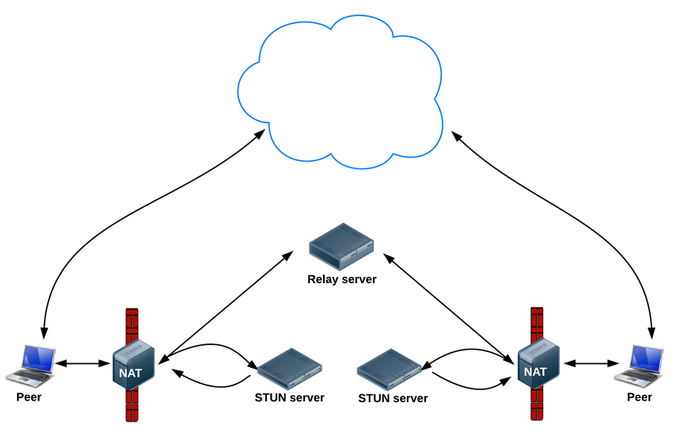
\includegraphics[height=0.30\textheight,natwidth=610,natheight=642]{figs/webrtc_network_finCandidate.png}
  	\caption{\gls{webrtc} Network: Finding connection candidates}
  	\label{fig:webrtc_network_finCandidate}
\end{figure} 

\begin{figure}
	\centering
    	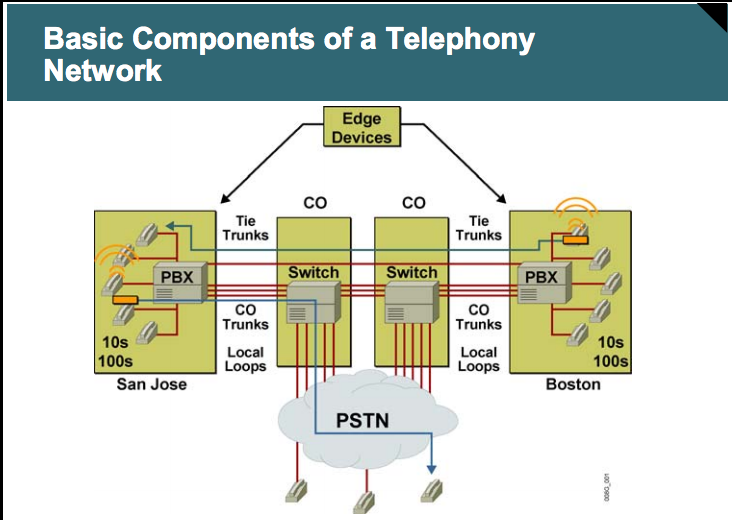
\includegraphics[height=0.40\textheight,natwidth=610,natheight=642]{figs/telephony_network.png}
  	\caption{Traditional Telephony Network}
  	\label{fig:telephony_network}
\end{figure}

\par Initially, \gls{ice} tries to connect peers directly, with the lowest possible latency, via \gls{udp}. In this process, \gls{stun} servers have a single task: to enable a peer behind a \gls{nat} to find out its public address and port. If \gls{udp} fails, \gls{ice} tries \gls{tcp}: first \gls{http}, then \gls{https}. If direct connection fails—in particular, because of enterprise \gls{nat} traversal and firewalls—\gls{ice} uses an intermediary (relay) \gls{turn} server. In other words, \gls{ice} will first use \gls{stun} with \gls{udp} to directly connect peers and, if that fails, will fall back to a \gls{turn} relay server. The expression 'finding candidates' refers to the process of finding network interfaces and ports.\cite{html5rock:webrtc}

\par The difference and usage of \gls{stun} server and \gls{turn} server will be discussed more detail in Chapter \ref{chp:sys_deploy}.

\par \gls{webrtc} needs server to help users discover each other and exchange 'real world' details such as names. Then \gls{webrtc} client applications (peers) exchange network information. After that, peers exchange data about media such as video format and resolution. Finally, \gls{webrtc} client applications can traverse \gls{nat} gateways and firewalls.

\par Compare to the traditional telephony network which is shown in Figure\ref{fig:telephony_network}\cite{web:teleVSvoip}, the main difference between these two communication network is that \gls{webrtc} is \gls{p2p} communication in \gls{stun} server scenario, after the signaling between end-peers, the media data are exchanged directly between tow peers. However, in the traditional telephony, all the media data are transferred to \gls{pbx} and switches regarding to \gls{pstn}\footnote{The PSTN consists of telephone lines, fiber optic cables, microwave transmission links, cellular networks, communications satellites, and undersea telephone cables, all interconnected by switching centers, thus allowing any telephone in the world to communicate with any other. Originally a network of fixed-line analog telephone systems, the PSTN is now almost entirely digital in its core network and includes mobile and other networks, as well as fixed telephones.\cite{wiki:pstn}} then reach the other side of the peer. Even in \gls{turn} server scenario for \gls{webrtc}, the media stream is only relaying to the \gls{turn} then directly transfer to another peer, no switches involved. Two server working scenario will be discussed in Chapter \ref{chp:sys_dev}.

\subsection{WebRTC Implementation Steps}

\begin{figure}
	\centering
    	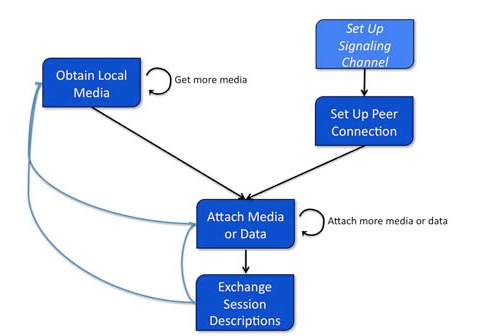
\includegraphics[width=0.80\textwidth,natwidth=610,natheight=642]{figs/webrtcApis.png}
  	\caption{WebRTC \gls{api} View with Signaling\cite{inbook:rtc-apis}}
  	\label{fig:webrtc_4steps}
\end{figure}

\noindent There are four main steps to implement a \gls{webrtc} session shown in Figure \ref{fig:webrtc_4steps}. The browser client need to obtain local media first, then set up a connection between the browser and the other peer through some signaling, after that attach the media and data channels to the connection, afterwards exchange the session description from each other. Finally the media stream will automatically exchange through the real-time peer to peer media channel.

\par Each step shown in the Figure \ref{fig:webrtc_4steps} is implemented by some \gls{webrtc} \gls{api}s. More detail about how to use \gls{webrtc} \gls{api}s to implement these steps will be covered in Chapter \ref{chp:sys_dev}. The \gls{webrtc} architecture is shown in Figure \ref{fig:webrtc_api_arch}, the main focus in this thesis will be Web \gls{api} part and transport part because Web \gls{api} is the tool to implement the \gls{webrtc} application and transport part is the key for \gls{webrtc} application to communicate with application server, media server and other end peer in the system. 

\begin{figure}
	\centering
    	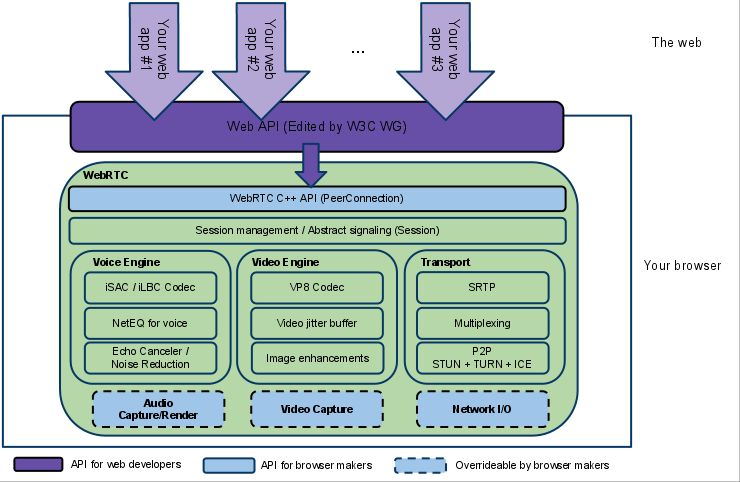
\includegraphics[width=0.80\textwidth,natwidth=610,natheight=642]{figs/WebRTCapiPic.png}
  	\caption{\gls{webrtc} architecture \cite{org:webrtc}}
  	\label{fig:webrtc_api_arch}
\end{figure}

\par Besides \gls{webrtc} \gls{api}s, signaling is the other important factor in the system. \gls{webrtc} uses \textit{RTCPeerConnection} (more about this \gls{api} will be discussed in Chapter \ref{chp:sys_dev}) to communicate streaming data between browsers, but also needs a mechanism to coordinate communication and to send control messages, a process known as signaling. Signaling methods and protocols are not specified by \gls{webrtc} by Google purpose, so signaling is not part of the \textit{RTCPeerConnection} \gls{api}.

\par Instead, \gls{webrtc} app developers can choose whatever messaging protocol they prefer, such as \gls{sip} or \gls{xmpp}, and any appropriate duplex (two-way) communication channel. The prototype application in this thesis will use WebSocket\footnote{WebSocket is a protocol providing full-duplex communications channels over a single TCP connection.\cite{wiki:websocket}} as signaling between \gls{webrtc} browser end point and keep use \gls{sip} as signaling for \gls{sip} end point (mobile/fixed phone based on \gls{pstn} in this case).

\noindent Signaling is used to exchange three types of information\cite{html5rock:webrtc}:

\begin{itemize}[topsep=-1em,parsep=0em,itemsep=0em]
 \item Session control messages: to initialize or close communication and report errors.
 \item Network configuration: to the outside world, the computer's IP address and port.
 \item Media capabilities: the codecs and resolutions can be handled by the browser and the browser it wants to communicate with.
\end{itemize}

\par The exchange of information via signaling must have completed successfully before peer-to-peer streaming can begin. For the prototype application in this thesis, the signaling has two mechanisms, one is for \gls{webrtc} browser clients and the other is for \gls{sip} clients, it will be explained in Chapter \ref{chp:sys_dev}.

\section{SIP}
\noindent The prototype application in this thesis will be integrated with \gls{pstn} through \gls{sip} server. Therefore the application server implemented in this system will use \gls{sip} signaling to communicate with \gls{sip} server to handle the signaling configuration with mobile/fixed phone end-point.

\subsection{What is SIP?}
\noindent The \gls{sip} is a signaling communications protocol, widely used for controlling multimedia communication sessions such as voice and video calls over \gls{ip} networks.

\par The protocol defines the messages that are sent between endpoints which govern establishment, termination and other essential elements of a call. \gls{sip} can be used for creating, modifying and terminating sessions consisting of one or several media streams. \gls{sip} can be used for two-party (unicast) or multiparty (multicast) sessions. Other \gls{sip} applications include video conferencing, streaming multimedia distribution, instant messaging, presence information, file transfer, fax over \gls{ip} and online games.\cite{wiki:sip}

\par \gls{sip} works in conjunction with several other application layer protocols that identify and carry the session media. Media identification and negotiation is achieved with the \gls{sdp}. It is different key filed format than the \gls{webrtc} \gls{sdp}. For the transmission of media streams (voice, video) \gls{sdp} typically employs the \gls{rtp} or \gls{srtp}. For secure transmissions of \gls{sip} messages, the protocol may be encrypted with \gls{tls}.

\subsection{SIP Network Elements}
\noindent In normal \gls{sip} network, \gls{sip} defines user-agents as well as several types of server network elements. Two \gls{sip} endpoints can communicate without any intervening \gls{sip} infrastructure. However, this approach is often impractical for a public service, which needs directory services to locate available nodes on the network. In the system implemented of this thesis, the application server will play as 'User Agent', 'Registrar' and 'Gateway' elements in the network.

\noindent \textbf{User Agent}\cite{wiki:sip}:
\par A \gls{sip} \gls{ua} is a logical network end-point used to create or receive \gls{sip} messages and thereby manage a \gls{sip} session. A \gls{sip} \gls{ua} can perform the role of a \gls{uac}, which sends \gls{sip} requests, and the \gls{uas}, which receives the requests and returns a \gls{sip} response. These roles of \gls{uac} and \gls{uas} only last for the duration of a \gls{sip} transaction.

\noindent \textbf{Registrar}\cite{wiki:sip}:
\par A registrar is a \gls{sip} endpoint that accepts REGISTER requests and places the information it receives in those requests into a location service for the domain it handles. The location service links one or more \gls{ip} addresses to the \gls{sip} \gls{uri} of the registering agent. The \gls{uri} uses the sip: scheme, although other protocol schemes are possible, such as tel:. More than one user agent can register at the same \gls{uri}, with the result that all registered user agents receive the calls to the \gls{uri}.

\noindent \textbf{Gateway}\cite{wiki:sip}:
\par Gateways can be used to interface a \gls{sip} network to other networks, such as the \gls{pstn}, which use different protocols or technologies. In the prototype application, the application server is the gateway to interface a \gls{webrtc} WebSocket network (The working process will be covered in Chapter \ref{chp:sys_dev}).

\subsection{SIP messages}
\noindent Since the application server in this system will be used as \gls{sip} \gls{ua} and \gls{sip} Gateway, it will send \gls{sip} message request to \gls{sip} server and receive \gls{sip} message request from the \gls{sip} server.

\par One of the wonderful things about \gls{sip} is that it is a text-based protocol modeled on the request/response model used in HTTP.  This makes it easy to debug because the messages are easy to construct and easy to see.  Contrasted with H.323\footnote{H.323 is a recommendation from the ITU Telecommunication Standardization Sector (ITU-T) that defines the protocols to provide audio-visual communication sessions on any packet network. The H.323 standard addresses call signaling and control, multimedia transport and control, and bandwidth control for point-to-point and multi-point conferences.\cite{wiki:h323}}, SIP is an exceedingly simple protocol.  Nevertheless, it has enough powerful features to model the behavior of a very complex traditional telephone \gls{pbx}.\cite{networkworld:sip}

\par There are two different types of \gls{sip} messages: requests and responses. The first line of a request has a method, defining the nature of the request, and a Request-URI, indicating where the request should be sent.The first line of a response has a response code.

\noindent For sip requests, regarding to RFC 3261\cite{rfc:3261}, the application server in the system will use following \gls{sip} messages:

\begin{itemize}[topsep=-1em,parsep=0em,itemsep=0em]
 \item \textbf{REGISTER:} Used by a \gls{ua} to indicate its current \gls{ip} address and the \gls{url}s for which it would like to receive calls.
 \item \textbf{INVITE:} Used to establish a media session between user agents.
 \item \textbf{ACK:} Confirms reliable message exchanges.
 \item \textbf{CANCEL:} Terminates a pending request.
 \item \textbf{BYE:} Terminates a session between two users in a conference.
\end{itemize}

\noindent The \gls{sip} response types defined in RFC 3261 will be listened by application server in the following response codes\cite{wiki:sip_response_codes}:

\begin{itemize}[topsep=-1em,parsep=0em,itemsep=0em]
 \item \textbf{100 Trying:} Extended search being performed may take a significant time so a forking proxy must send a 100 Trying response.
 \item \textbf{180 Ringing:} Destination user agent received INVITE, and is alerting user of call.
 \item \textbf{200 OK:} Indicates the request was successful.
 \item \textbf{400 Bad Request:} The request could not be understood due to malformed syntax.
 \item \textbf{401 Unauthorized:} The request requires user authentication. This response is issued by \gls{uas}s and registrars.
 \item \textbf{408 Request Timeout:} Couldn't find the user in time. The server could not produce a response within a suitable amount of time, for example, if it could not determine the location of the user in time. The client MAY repeat the request without modifications at any later time.
 \item \textbf{480 Temporarily Unavailable:} Callee currently unavailable.
 \item \textbf{486 Busy Here:} Callee is busy.
\end{itemize}

\par By listening these \gls{sip} response, the application will send request to either \gls{webrtc} browser client or \gls{sip} client to play as the gateway role in the system. This gateway mechanism will be introduced in Chapter \ref{chp:sys_dev}.

\section{Prototype System Working Flow}
\noindent The main purpose of this thesis is to make unified communication solution with \gls{webrtc} technology. 
\par To connect with the traditional telephony network, the \gls{voip} system bridges the \gls{pstn} and the \gls{ip} network. \gls{voip} systems employ session control and signaling protocols to control the signaling, set-up, and tear-down of calls. They transport audio streams over \gls{ip} networks using special media delivery protocols that encode voice, audio, video with audio codecs, and video codecs as Digital audio by streaming media. In this prototype, \gls{sip} signaling is used because of its widely usage and current target \gls{pstn} has \gls{sip} server support.

\begin{figure}
	\centering
    	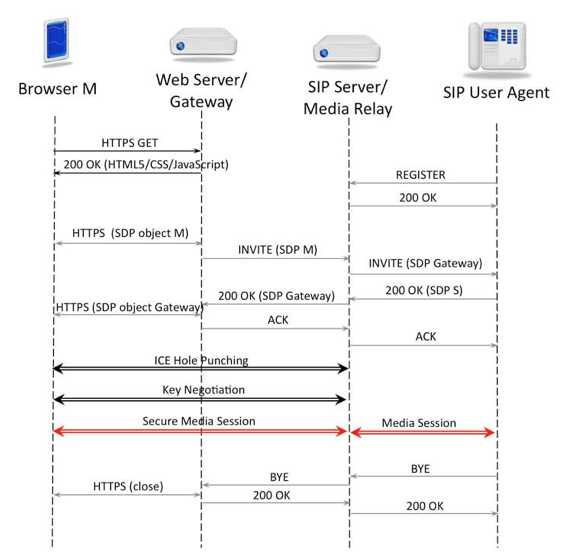
\includegraphics[width=0.60\textheight,natwidth=610,natheight=642]{figs/system_work_flow.png}
  	\caption{Prototype System Working Diagram \cite{inbook:sys_work_diagram}}
  	\label{fig:sys_work_diagram}
\end{figure}

\par The Figure \ref{fig:sys_work_diagram} shows the basic working flow of the prototype system. The Web Server is the application server in the system, it mainly bridges the \gls{webrtc} browser client with other \gls{webrtc} clients and the \gls{sip} network. The \gls{sip} server bridges the \gls{sip} network and \gls{pstn} network or traditional telephony network. And also the Media Relay server relay all the media stream from different end clients, in the prototype system, it is a media server provided by Dialogic, the Network Fuel company, which is called PowerMedia XMS v2.1\footnote{PowerMedia XMS is pre-integrated with a variety of application servers and signaling gateways with HTTP-to-SIP (H2S) functionality and rapidly integrates with others using its web API or standard interfaces.} PowerMedia XMS acts as a WebRTC Media Gateway to mediate WebRTC media-plane differences from those of typical existing VoIP networks including encryption interworking, transcoding, and client-based NAT traversal support. The reason to use this media server is to avoid hard-code transition between \gls{webrtc} \gls{sdp} and \gls{sip} \gls{sdp}. Then the end client no matter it is \gls{webrtc} client or \gls{sip} client, they will communicate with the same signaling client for their aspect.
\par Moreover, since the media server is used in this case, during the multiple end-point conversation, each end-point will only exchange their media stream to the single end-point on the media server (PowerMedia XMS server), it will make light client and centralized server control. The benefit of this system architecture will be discussed more in the Chapter \ref{chp:sys_dev}.

\par Therefore, in the Figure \ref{fig:sys_work_diagram}, all the end point keep using their own original signaling protocol to communicate with different server in order to reach different scope end point.
\chapter{Prototype System Development}
\label{chp:sys_dev}

\noindent In this chapter, it will cover development implementation progress of the prototype system along with explanation and analysis. The prototype system is designed based on preliminary studies from previous chapter. There will be different implementation solutions to the prototype working scenario  discussed and evaluated in this chapter. After evaluating these solutions, it will come up with the fit solution to the prototype working scenario. 

\section{Prototype System Network}

\noindent In the original \gls{webrtc} application implementation, it uses mesh network because \gls{webrtc} means to be the peer to peer communication method bypass the third party server. However, the prototype system will use centralized server network to control and route the communication channels between different types end points. In this section, it will describe the reason to use centralized server network rather than mesh network.

\subsection{Mesh Network}

\subsection{Centralized Server Network}

\section{WebRTC APIs Implementation}

\noindent \gls{webrtc} components are accessed with JavaScript APIs. Currently in development are the Network Stream \gls{api}, which represents an audio or video data stream, and the PeerConnection \gls{api}, which allows two or more users to communicate browser-to-browser. Also under development is a DataChannel \gls{api} that enables communication of other types of data for real-time gaming, text chat, file transfer, and so forth. Because the media server used in prototype system is not support for DataChannel yet, the DataChannel \gls{api} will not be covered in this section.

\begin{figure}
	\centering
    	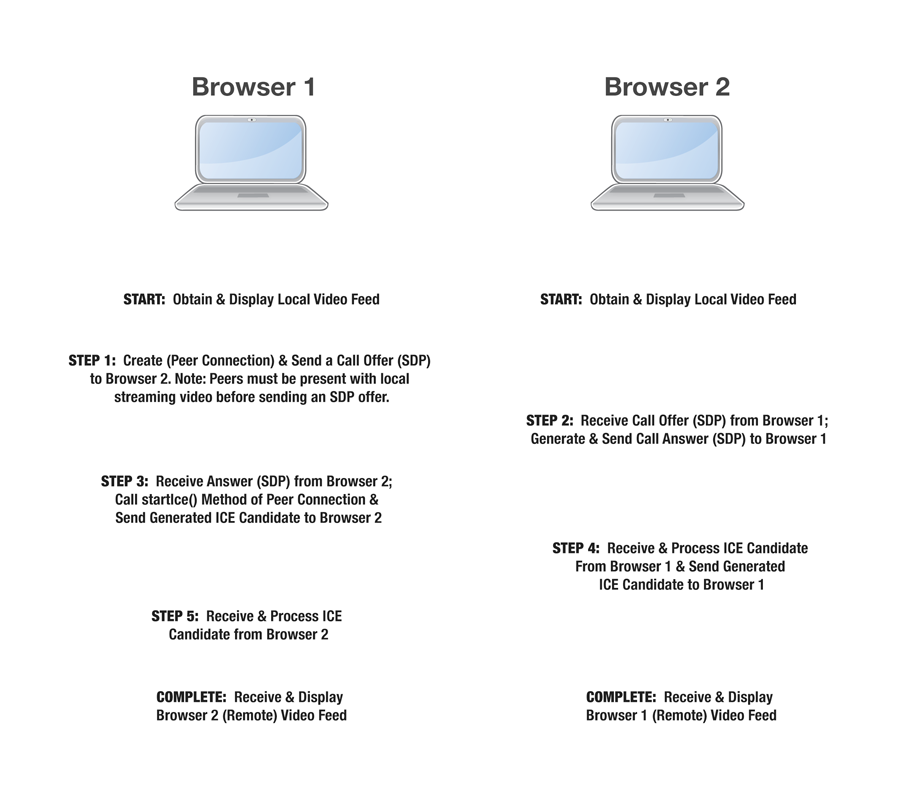
\includegraphics[height=0.50\textheight,natwidth=610,natheight=642]{figs/webrtc_diagram.png}
  	\caption{WebRTC two peer communication process\cite{mdn:p2pwebrtc}}
  	\label{fig:webrtc_diagram}
\end{figure}

\subsection{MediaStream API}

\par The MediaStream \gls{api} represents synchronized streams of media. For example, a stream taken from camera and microphone input has synchronized video and audio tracks. In order to obtain local media, the start step for both peers in Figure \ref{fig:webrtc_diagram} which is a communication process to set up call process from caller peer, the \gls{webrtc} \gls{api}s provide \textit{navigator.getUserMedia()} function to get the video and audio stream from user. For privacy reasons, a web application’s request for access to a user’s microphone or camera will only be granted after the browser has obtained permission from the user. Each MediaStream has an input, which might be a MediaStream generated by \textit{navigator.getUserMedia()}, and an output, which might be passed to a video element or an \textit{RTCPeerConnection}.
\par The \textit{getUserMedia()} method takes three parameters:

\begin{itemize}[topsep=-1em,parsep=0em,itemsep=0em]
 \item A constraints object.
 \item A success callback which, if called, is passed a MediaStream.
 \item A failure callback which, if called, is passed an error object.
\end{itemize}

\par The Code Snippet \ref{code:get_user_media} shows that how the prototype application implements \textit{getUserMedia()} function, it is encapsulated in \textit{WebRTCService} (service is a reusable business logic independent of views in prototype application regarding to AngularJs framework\footnote{AngularJS is an open-source web application framework, maintained by Google and community, that assists with creating single-page applications, one-page web applications that only require HTML, CSS, and JavaScript on the client side.\cite{wiki:angularjs}}). There will be more discuss about prototype application framework in the later part of this chapter. For the constraints object in parameters, the prototype application set 'audio' and 'video' value to true because it is necessary for the real-time communication application to have video and audio stream both.

\begin{lstlisting}[caption={Get User Media Stream function},label={code:get_user_media}]
var media_constraints = {audio: true,video: true};

function _setMediaStream(){
	WebRTCService.getUserMedia(media_constraints,
  								_handleUserMedia,
  								_handleUserMediaError);
  	console.log('Getting user media with constraints', 
  				media_constraints);
}
\end{lstlisting}

\par \textit{getUserMedia()} function is currently available in Chrome, Opera and Firefox. Almost all of the \gls{webrtc} \gls{api}s are slightly different based on different browsers implementation. In the Code Snippet \ref{code:webrtc_service}, from line 40 to line 103 is to make all the set up process for FireFox and from line 106 to line 175 is to make the same set up process for Google Chrome. Because \gls{webrtc} is not standard Web \gls{api} yet, so the implementation on different browsers are different and the \gls{webrtc} \gls{api}s names are slightly different in some browsers. For example, in the Code Snippet \ref{code:webrtc_service} showing, the \textit{RTCPeerConnection} \gls{api} in Firefox is \textit{mozRTCPeerConnection} but in Google Chrome it is \textit{webkitRTCPeerConnection}. In order to make the \gls{webrtc} application works on more browsers, the client side need to figure out which kind of browser is using on the machine then call the corresponding \gls{webrtc} \gls{api}s. Google provides a JavaScript shim called \textit{adapter.js}. It is maintained by Google, it abstracts away browser differences and spec changes. For Angularjs framework used by prototype application, then the \textit{WebRTCService} is implemented to be integrated with \textit{adapter.js} function to achieve the goal of compatibility.

\par However, the prototype application in this thesis will only focus on Google Chrome browser\footnote{Google Chrome is a freeware web browser developed by Google. It used the WebKit layout engine until version 27 and, with the exception of its iOS releases, from version 28 and beyond uses the WebKit fork Blink.\cite{wiki:google_chrome}} to simplify the development process because \gls{webrtc} lower level implementation on different browser s are different and hard to track the issues. Then most of the results in this thesis is based on the application performance of Google Chrome browser. The reason to choose Google Chrome browser rather than other browser because \gls{webrtc} is the technology rapidly pushed by Google and Google Chrome browser has the most market share in the world. As of March 2014, StatCounter estimates that Google Chrome has a 43\% worldwide usage share of web browsers, making it the most widely used web browser in the world.\cite{wiki:google_chrome} However, Google changes a lot to improve the performance of \gls{webrtc} on Google Chrome browser, then it makes the \gls{webrtc} \gls{api}s work different on different version of Google Chrome browser. In the Code Snippet \ref{code:webrtc_service}, from line 124 to line line 136 is the sample case to distinguish the difference among different version of Google Chrome to handle the \textit{RTCPeerConnection} \gls{ice} server constraint implementation.

\par Since \gls{webrtc} \gls{api}s is not standard \gls{api} yet, the prototype application in this thesis will not pay too much work-load on compatibility for different browsers platform. More detail about this issue will be discussed in the Chapter \ref{chp:future_work}.

\subsection{RTCPeerConnection API}

\noindent To set up peer connection, the \textit{RTCPeerConnection} \gls{api} sets up a connection between two peers. In this context, “peers” means two communication endpoints on the World Wide Web. Instead of requiring communication through a server, the communication is direct between the two entities. In the specific case of \gls{webrtc}, a peer connection is a direct media connection between two web browsers. This is particularly relevant when a multi-way communication such as a conference call is set up among three or more browsers. Each pair of browsers will require a single peer connection to join them, allowing for audio and video media to flow directly between the two peers. 

\par To establish peer connection, it requires a new \textit{RTCPeerConnection} object. The only input to the \textit{RTCPeerConnection} constructor method is a configuration object containing the information that \gls{ice}, will use to “punch holes” through intervening \gls{nat} devices and firewalls. The Code Snippet \ref{code:create_peer_connection} shows the create \textit{RTCPeerConnection} object and set three listener (\textit{onicecandidate},\textit{onaddstream},\textit{onremovestream}) to trigger the handlers to deal with the \gls{ice} candidate event and remote stream add/remove events.

\par The \textit{RTCPeerConnection} \gls{api} has two arguments to set, one is configuration object for peer connection and the other is constraint object (set transparent protocol and encryption) for peer connection, these value are shown in Code Snippet \ref{code:create_peer_connection} line 1 to line 10. In the showing case, the prototype is using \gls{stun} servers for different browser aspect, and set the \gls{rtc} channel encryption protocol to \gls{dtls}\footnote{In information technology, the Datagram Transport Layer Security (DTLS) protocol provides communications privacy for datagram protocols. DTLS allows datagram-based applications to communicate in a way that is designed to prevent eavesdropping, tampering, or message forgery.\cite{wiki:dtls}} and enable the \gls{rtc} DataChannel.

\par Because in Firefox, \gls{webrtc} media transparent channel is only based on \gls{dtls} protocol, and in latest version Google Chrome, it is support, then in the prototype application, it will use \gls{dtls} protocol to exchange the media stream.

\par There are two \gls{api}s to handle the \textit{IceCandidate} object which contains \gls{ice} information data. One is \textit{onicecandidate} listener to trigger the function to handle the new \textit{IceCandidate} data object. The other one is \textit{addIceCandidate} function, which is shown in the Code Snippet \ref{code:add_remote_ice}, to add the new \textit{IceCandidate} data object to the remote/local peer connection session description field. 

\begin{lstlisting}[caption={Create Peer Connection function},label={code:create_peer_connection}]
pc_config = WebRTCService.webrtcDetectedBrowser() === 'firefox' ?
  			{'iceServers':[{'urls':'stun:stun.services.mozilla.com'}]} :
  			{'iceServers':[{'urls': 'stun:stun.l.google.com:19302'}]};

pc_constraints = {
			  'optional': [
			    {'DtlsSrtpKeyAgreement': true},
			    {'RtpDataChannels': true}
			  ]
			};
			
function _createPeerConnection(){

	try {
		pc = WebRTCService.peerConnection(pc_config, pc_constraints);
		pc.onicecandidate = _handleIceCandidate;
		console.log('Created RTCPeerConnnection with:\n' +
		      '  config: \'' + JSON.stringify(pc_config) + '\';\n' +
		      '  constraints: \'' + JSON.stringify(pc_constraints) + '\'.');
	} catch (e) {
		console.log('Failed to create PeerConnection, exception: ' + e.message);
		alert('Cannot create RTCPeerConnection object.');
		return;
	}
	pc.onaddstream = _handleRemoteStreamAdded;
	pc.onremovestream = _handleRemoteStreamRemoved;

}
\end{lstlisting}

\begin{lstlisting}[caption={Add Remote IceCandidate function},label={code:add_remote_ice}]
var candidate = WebRTCService.RTCIceCandidate({
					    	sdpMLineIndex:data.content.label,
					    	sdpMid:data.content.id,
					    candidate:data.content.candidate
				});
pc.addIceCandidate(candidate);

\end{lstlisting}

\par In the step 2 of Figure \ref{fig:webrtc_diagram}, after the caller \textit{RTCPeerConnection} run \textit{createOffer()} function to send offer to callee through signaling channel, the callee need run \textit{createAnswer()} function to ask the \gls{stun}/\gls{turn} server to find the path for each other peer and create the answer with \gls{sdp} content. \gls{sdp} is intended for describing multimedia communication sessions for the purposes of session announcement, session invitation, and parameter negotiation. \gls{sdp} does not deliver media itself but is used for negotiation between end points of media type, format, and all associated properties.\cite{wiki:sdp} Before \textit{RTCPeerConnection} use \textit{createOffer()} function to send a \gls{webrtc} offer to the callee, it is required to be present with local streaming video, like Figure \ref{fig:webrtc_diagram} mentioned.

\par The sample \gls{sdp} from the prototype application is shown in Code Snippet \ref{log:webrtc_answer_sdp}. Line 2 in Code Snippet \ref{log:webrtc_answer_sdp} is the field 'o', it describes originator, session identifier, username, id, version number and network address. It usually means that where this package comes from. Line 7 and line 17 are field 'm', it describes media name and transport address. And line 11,12 and line 27,28 are the relevant lines for audio and video media field, they describes media filed 'candidate' attributes, in the sample case of Code Snippet \ref{log:webrtc_answer_sdp}, they are the \gls{ice} candidate from the \gls{stun}/\gls{turn} server. These are important fields regarding to the prototype system because they are used in XMS server and application server of the prototype system.

\begin{lstlisting}[caption={Sample \gls{webrtc} Answer \gls{sdp}},label={log:webrtc_answer_sdp}]
sdp: v=0
o=xmserver 1399363527 1399363528 IN IP4 10.254.9.135
s=xmserver
c=IN IP4 10.254.9.135
t=0 0
a=ice-lite
m=audio 49152 RTP/SAVPF 0 126
a=rtpmap:0 PCMU/8000
a=sendrecv
a=rtcp:49153
a=candidate:1 1 UDP 2130706431 10.254.9.135 49152 typ host
a=candidate:1 2 UDP 2130706430 10.254.9.135 49153 typ host
...
a=acfg:1 t=1
a=rtpmap:126 telephone-event/8000
a=fmtp:126 0-15
m=video 57344 RTP/SAVPF 100
b=AS:1000
a=rtpmap:100 VP8/90000
a=fmtp:100 max-fr=30; max-fs=1200
a=sendrecv
a=rtcp:57345
a=rtcp-fb:100 ccm fir
a=rtcp-fb:100 nack
a=rtcp-fb:100 nack pli
a=rtcp-fb:100 goog-remb
a=candidate:2 1 UDP 2130706431 10.254.9.135 57344 typ host
a=candidate:2 2 UDP 2130706430 10.254.9.135 57345 typ host
...
\end{lstlisting}

\par In the step 3 of Figure \ref{fig:webrtc_diagram}, the caller will receive the answer from callee and process it by adding the remote \gls{sdp} to \textit{RTCPeerConnection}, like the Code Snippet \ref{code:add_remote_ice}. By the meantime, the step 4 of Figure \ref{fig:webrtc_diagram}, the callee will receive the \gls{sdp} from caller with the \gls{ice} candidate information data, and process it the same way as caller does, add some to \textit{RTCPeerConnection} object by \textit{addIceCandidate()} function.

\par \gls{webrtc} clients (known as peers) also need to ascertain and exchange local and remote audio and video media information, such as resolution and codec capabilities. Signaling to exchange media configuration information proceeds by exchanging an offer and an answer using the \gls{sdp}. The \textit{createOffer()} function and \textit{createAnswer()} function both have callback function to handle the \gls{sdp} either to call \textit{setLocalDescription()} by caller or call \textit{setRemoteDescription()} by callee when callee gets the caller's \gls{sdp} from \gls{webrtc} offer. The Code Snippet\ref{log:webrtc_answer_sdp} shown is the \gls{webrtc} answer \gls{sdp} from the callee when the callee end-point decide to accept this conversion session.

\par Once the \textit{RTCPeerConnection} is established, the client need configure where the media or data to store and display if it is necessary. In the prototype application of this thesis, media stream will be displayed in a \gls{html5} tag called \textit{<video>}. It will only be shown when there is media stream in \textit{<video>} tag source.

\section{Prototype Implementation Framework}

\noindent Since \gls{webrtc} is a web \gls{api}, the prototype application will be a web application. There are many different web application framework nowadays to provide rich-client web application. In this section, some of the web application framework will be discussed to figure out which framework is best solution to the prototype scenario. Furthermore, application server will be discussed with different implementation solutions since it does signaling and bridge the \gls{sip} network and clients.

\subsection{Client Implementation Framework}

\noindent To choose web application framework to implement the client application in this thesis scenario, the main fact is that if the web  application framework is fit to the real time communication application and if the framework has the ability to integrate with \gls{webrtc} \gls{api}. After research about these kinds of web application framework, it narrows down to three main framework to discuss.

\textbf{AngularDart :}

\par AngularDart is a framework for building web-apps in Dart. Dart is an open-source Web programming language developed by Google. It is a class-based, single inheritance, object-oriented language with C-style syntax. It supports interfaces, abstract classes, reified generics, and optional typing. Static type annotations do not affect the runtime semantics of the code. Instead, the type annotations can provide documentation for tools like static checkers and dynamic run time checks.\cite{wiki:dart} Because most of the script language is not type strict, it is easy to mess up the code and value type in script language. Moreover, Dart has Dart-to-JavaScript compiler,dart2js, it makes Dart can be used in client and server both. Addition to AngularJs framework in Dart, it provide a professional web application structure to the developer to implement. More about AngularJs notable features will be covered in the later AngularJs solutions. 

\par The \gls{webrtc} implementation in Dart is in this repository: \url{https://github.com/br1anchen/AngularDart_webRTC}. The Code Snippet \ref{code:dart_webrtcctrl} shows the main controller in AngularDart. The line 5 is to import \gls{webrtc} client class \textit{speack\_client.dart}, the class has all the \gls{webrtc} \gls{api}s implemented in Dart. Line 23 is to initialize the \textit{SpeakerClient} object and set the arguments WebSocket url and room name. They are used for signaling in WebSocket Protocol.

\par However, after implementation of client application and server back-end in Dart. There is a critical bug in the current Dartium browser. The Dart SDK ships with a version of the Chromium web browser modified to include a Dart \gls{vm}. Dartium browser can run Dart code directly without compilation to JavaScript. It is intended as a development tool for Dart applications, rather than as a general purpose web browser. When embedding Dart code into web apps, the current recommended procedure is to load a bootstrap JavaScript file, "dart.js", which will detect the presence or absence of the Dart \gls{vm} and load the corresponding Dart or compiled JavaScript code, respectively, therefore guaranteeing browser compatibility with or without the custom Dart VM.\cite{wiki:dart} 
\par The issue noticed as \textbf{RtcPeerConnection.addIceCandidate results in a NotSupportedError: Internal Dartium Exception} in the Dart Google Project issues.\cite{bug:dartium} The sample code in the \gls{webrtc} Dart implementation shown in Code Snippet \ref{code:dart_add_ice}, line 1 is to create \textit{RTCPeerConnection} object. From line 5 to line 13 is to send message to server when \textit{RTCPeerConnection} object get \textit{onIceCandidate} event witch \gls{ice} candidate information. Line 17 is to bind the message listener event to Dart function \textit{onCandidate.listen}. From line 21 to line 30 is the Dart function to create \textit{RTCIceCandidate} object and add to \textit{RTCPeerConnection} object. The bug issue happens on line 27, when the \textit{RTCPeerConnection} call \textit{addIceCandidate} function, it is not allowed to have callback function in current version Dartium.

\begin{lstlisting}[caption={Add IceCandidate in Dart},label={code:dart_add_ice}]
var pc = new RtcPeerConnection(_iceServers, _dataConfig);

....

    pc.onIceCandidate.listen((e){
      if (e.candidate != null) {
        _send('candidate', {
          'label': e.candidate.sdpMLineIndex,
          'id': id,
          'candidate': e.candidate.candidate
        });
      }
    });
    
...

get onCandidate => _messages.where((m) => m['type'] == 'candidate');

...

onCandidate.listen((message) {
	var candidate = new RtcIceCandidate({
		'sdpMLineIndex': message['label'],
        'candidate': message['candidate']
    });

    _connections[message['id']].addIceCandidate(candidate,(){},(e){
    		print('add ice candidate error');
    });
});

...
\end{lstlisting}

\par There is a work around solution in one Stack Overflow\footnote{Stack Overflow is a privately held website, the flagship site of the Stack Exchange Network, created in 2008 by Jeff Atwood and Joel Spolsky, as a more open alternative to earlier Q\&A sites such as Experts Exchange.} answer: \url{http://stackoverflow.com/questions/20404312/how-to-call-addicecandidate-in-dart}. The fix method is to use \textit{js-interop} library to use pure JavaScript code in Dart to call the \gls{webrtc} Web \gls{api} instead of Dart \gls{webrtc} interface.
\par Mozilla's Brendan Eich, who developed the JavaScript language, stated that:

\textit{"I guarantee you that Apple and Microsoft (and Opera and Mozilla, but the first two are enough) will never embed the Dart VM. So 'Works best in Chrome' and even 'Works only in Chrome' are new norms promulgated intentionally by Google. We see more of this fragmentation every day. As a user of Chrome and Firefox (and Safari), I find it painful to experience, never mind the political bad taste."}\cite{wiki:dart}

\par Since Dart in not support to most modern web browser like FireFox, will not be used in this prototype.

\textbf{Sipml5 + webrtc2sip:}

\begin{figure}
	\centering
    	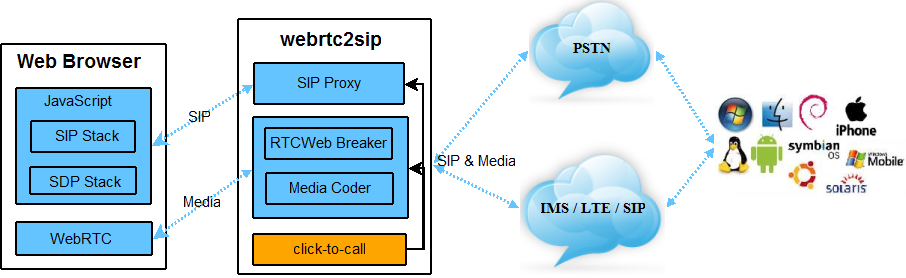
\includegraphics[width=0.80\textwidth,natwidth=610,natheight=642]{figs/sipml5_network.png}
  	\caption{Sipml5 and webrtc2sip Network}
  	\label{fig:sipml5_network}
\end{figure}

\par Sipml5 is the world's first open source \gls{html5} \gls{sip} client entirely written in JavaScript for integration in social networks (FaceBook, Twitter, Google+), online games, e-commerce websites, email signatures. The media stack rely on \gls{webrtc}. The client can be used to connect to any \gls{sip} or \gls{ims} network from your preferred browser to make and receive audio/video calls and instant messages.\cite{website:sipml5}

\par Sipml5 provides whole client solution to communicate with other kind of signaling real-time communication network. The \gls{sip} and \gls{sdp} stacks are entirely written in JavaScript and the network transport uses WebSockets as per draft-ibc-sipcore-sip-websocket. However the community of sipml5 is not so active, the issues and source code on sipml5 source code project website \url{https://code.google.com/p/sipml5/} are not updated regularly. Like the Figure \ref{fig:sipml5_network} showing, it works with media gateway webrtc2sip.

\par webrtc2sip is a smart and powerful gateway using \gls{webrtc} and \gls{sip} to turn your browser into a phone with audio, video and \gls{sms} capabilities. The gateway allows your web browser to make and receive calls from/to any \gls{sip}-legacy network or \gls{pstn}.
The gateway contains four modules: \gls{sip} Proxy, RTCWeb Breaker, Media Coder, Click-to-Call.\cite{website:webrtc2sip}

\par In the prototype working scenario, it is necessary to have media gateway to communicate with \gls{sip}-legacy network. Since the current \gls{pstn} using in this prototype go through Gintel \gls{mpbx} Platform, it is necessary to use RTCWeb Breaker to be able to connect the browser to a SIP-legacy endpoint.

\par Therefore, the test for Sipml5 and webrtc2sip solution is based on the live demo \url{http://sipml5.org/call.htm}. But even with the RTCWeb Breaker, the test is still failed to call any number through the target \gls{pstn}. Since most of the source code of these two framework are hidden from the encapsulation, it is impossible to debug which part of the testing system is the problem. In the test, the registration for \gls{sip} client is successful, but there are 'too long message' in the \gls{sip} error message got from the \gls{sip} server. It means that the sipml5 and webrtc2sip network architecture is not compatible with the target \gls{pstn} through the Gintel \gls{mpbx} Platform. This solution can not be used in the prototype system.

\textbf{AngularJs + Socket.IO:}

\par AngularJS is built around the belief that declarative programming should be used for building user interfaces and wiring software components, while imperative programming is excellent for expressing business logic. The framework adapts and extends traditional \gls{html} to better serve dynamic content through two-way data-binding that allows for the automatic synchronization of models and views. As a result, AngularJS de-emphasizes \gls{dom} manipulation and improves testability. Angular follows the \gls{mvc} pattern of software engineering and encourages loose coupling between presentation, data, and logic components. Using dependency injection, Angular brings traditional server-side services, such as view-dependent controllers, to client-side web applications. Consequently, much of the burden on the backend is reduced, leading to much lighter web applications.\cite{wiki:angularjs}

\par AngularJs is perfect for single-page web application, the framework features provide developer a professional way to structure the web application in JavaScript. Moreover, the developer community of AngularJs is quite active, there are a lot of different Angular module services to provide the different interfaces against different web \gls{api}s.In the prototype, there will be several third party Angular module library to be used in order to integrate with some advanced JavaScript library or web \gls{api}s in Angular style.

\par Socket.IO is a JavaScript library for realtime web applications. It has two parts: a client-side library that runs in the browser, and a server-side library for node.js. Both components have a nearly identical \gls{api}. Socket.IO primarily uses the WebSocket protocol, but if needed can fallback on multiple other methods, such as Adobe Flash sockets, \gls{jsonp} polling, and \gls{ajax} long polling, while providing the same interface. Although it can be used as simply a wrapper for WebSocket, it provides many more features, including broadcasting to multiple sockets, storing data associated with each client, and asynchronous I/O.\cite{wiki:socketio} In the prototype application, Socket.IO is used in WebSocket protocol because the WebSocket protocol provides full-duplex communications channels over a single \gls{tcp} connection. Then the communication channel will be active and real time between the clients and server during the whole connecting procedure. It fits the real time communication application requirement.

\par After test demo client application implemented in AngularJs and Socket.IO frameworks, it works fine with the basic \gls{webrtc} functions and simple \gls{sip} registration against \gls{sip} server to target \gls{pstn}. The final decision of the client implementation framework of prototype system will be AngularJs and Socket.IO.

\subsection{Server Implementation Framework}

\noindent Since the client side will use Socket.IO as communication protocol library, the server back-end in the prototype system will use Node.js as server implementation framework. In thist section, more detail about comparison and differences of Node.js against traditional web service back-end (in Java, ASP .NET or \gls{php}) will be covered.

\textbf{Node.js:}

\par 

\textbf{Mobicents Sip Servlets + Java web service:}

\par 
\chapter{Prototype System Deployment}
\label{chp:sys_deploy}

\noindent In this Chapter, there will be three main topics discussed because of deploying the prototype system to production usage.

\section{TURN Server Deployment}

\par During the development of the prototype system, the test based on XMS media server is not stable at the beginning. There is one way audio issue happens in the prototype system when \gls{webrtc} client init a outbound call to a \gls{sip} client(mobile phone). Since it is working fine when the outbound \gls{sip} client call into the \gls{webrtc} client, after tracing the network log from the XMS media server, the problem is the \gls{ice} candidate information got from the original \gls{stun} server can not punch the whole on the firewall of the XMS media server. It is normal to replace the \gls{stun} server as \gls{turn} server to solve this problem because if the \gls{stun} server way is blocked during the media stream exchange from two end point, it will switch to \gls{turn} server way to exchange the media stream through the \gls{turn} server to rely all the media traffic.

\par Moreover, the \gls{turn} server solution will work well in the different corporation networks scenario since there will be highly restrict corporation firewall in front of the corporation network. Then \gls{turn} server can rely all the media stream to establish the peer to peer connection. After testing prototype system against \gls{turn} server instead of \gls{stun} server provided by Google (shown at line 3 in Code Snippet \ref{code:create_peer_connection}), the one way audio issue is solved and two end client in different corporation network scenario works fine as well.

\par To set up \gls{turn} server in the production of prototype system, the prototype system uses \gls{aws} \gls{ec2}\footnote{Amazon Elastic Compute Cloud (EC2) is a central part of Amazon.com's cloud computing platform, Amazon Web Services (AWS). EC2 allows users to rent virtual computers on which to run their own computer applications. EC2 allows scalable deployment of applications by providing a Web service through which a user can boot an Amazon Machine Image to create a virtual machine, which Amazon calls an "instance", containing any software desired. A user can create, launch, and terminate server instances as needed, paying by the hour for active servers, hence the term "elastic". EC2 provides users with control over the geographical location of instances that allows for latency optimization and high levels of redundancy.\cite{wiki:ec2}}, \gls{ip} address: 54.187.157.224. There is a free open source implementation of \gls{turn} and \gls{stun} server maintained by Google. It provides the \gls{aws} \gls{ec2} hosting image, then it is only necessary to configure the \gls{aws} \gls{ec2} virtual instance to open the necessary ports for the \gls{turn} server usage. It is shown in the following list:
\begin{itemize}[topsep=-1em,parsep=0em,itemsep=0em]
 \item TCP 443
 \item TCP 3478-3479
 \item TCP 32355-65535
 \item UDP 3478-3479
 \item UDP 32355-65535
\end{itemize}

\par Moreover, the \gls{turn} server can either use a flat file or a \gls{sql} database for configuration and user information. In the prototype system, the \gls{turn} server on \gls{aws} \gls{ec2} will use a flat file for configuration and user information. It is edited in "/usr/local/etc/turnuserdb.conf" by adding an entry on its own line: "my\_username:my\_password".\cite{dialogic:turn} Other configurations need to be completed by following the README file under the hosting instance image directory on \gls{aws} \gls{ec2}. There are several paramters need to be set in "/etc/turnserver.conf" on \gls{turn} server.

\par Besides establishment for \gls{turn} server, there are some changes need to be done on the client application as well in order to use this \gls{turn} server to fetch the useful \gls{ice} candidate information during the peer to peer connection. Compare to the Code Snippet \ref{code:create_peer_connection} with original Google \gls{stun} server address, in Code Snippet \ref{code:client_turn_server}, prototype \gls{turn} server is set as \textit{iceServer}. The \textit{iceTransports} field is the parameter to force client to use \gls{turn} server but it is only purposed by Google Chrome, it is not standard and it is not implemented in Google Chrome yet.

\begin{lstlisting}[caption={Using TURN Server on WebRTC Client},label={code:client_turn_server}]
if (location.hostname != "localhost") {
  			
				pc_config = 
				{
					'iceServers': [{
						'urls': 'turn:54.187.157.224',
						'username': 'my_username',
						'credential': 'my_password'
					}],
					'iceTransports': 'relay'
				};
			}
\end{lstlisting}


\section{Application Server Deployment}

\par Because the prototype application server is implemented in Node.js, there is no restrict requirements for the operation system platform to deploy the application server if the operation system can install Node.js library and can run V8 JavaScript Engine\footnote{The V8 JavaScript Engine is an open source JavaScript engine developed by Google for the Google Chrome web browser.V8 compiles JavaScript to native machine code (IA-32, x86-64, ARM, or MIPS ISAs) before executing it, instead of more traditional techniques such as interpreting bytecode or compiling whole program to machine code and executing it from a filesystem. \cite{wiki:v8}}.

\par It also needs to open the \textit{5060} port to support \gls{udp} for \gls{sip} stack usage. Then it just need to use \textit{node server.js} command to host the application server for production.

\section{XMS Server Deployment}

\par The XMS media server is host on a stand alone machine during the development. For deployment reason, it is necessary to map the internal \gls{ip} address of XMS media server to a public \gls{ip} address. And it is important to open the necessary port for the XMS media usage. According to the documentation of Dialogic PowerMedia XMS 
Installation and Configuration Guide\cite{dialogic:xms_install},the default PowerMedia XMS configuration uses the following ports:
\begin{itemize}[topsep=-1em,parsep=0em,itemsep=0em]
 \item \gls{tcp}: 22, 80, 81, 443, 5060, 1080, 15001 
 \item \gls{udp}: 5060, 49152-53152, 57344-57840 
\end{itemize}

\par Because the application server and XMS media server in the prototype system are host in the corporation network, it only opens necessary port to the public network. During the exchange \gls{ice} candidate information for client, the XMS \gls{ip} address will be the internal \gls{ip} address by the rule of the corporation network. It is necessary to change the internal \gls{ip} address into public \gls{ip} address before pushing the \gls{ice} candidate information back to the end point client. This process is implemented at line 29 in Code Snippet \ref{code:xms}, it simply just replaces the internal \gls{ip} address as public \gls{ip} address of XMS media server in the \gls{sdp} content string.


\chapter{Discussion and Conclusion}
\label{chp:future_work}

\noindent In this Chapter, there are some future improvements discussion for the prototype system will be discussed. And some future research directions of \gls{webrtc} integrated with traditional telephony network will be include as well.

\section{Future Work}

\subsection{RTCDataChannel usage}

\par The \textit{RTCDataChannel} \gls{api} enables peer-to-peer exchange of arbitrary data, with low latency and high throughput.The API has several features to make the most of \textit{RTCPeerConnection} and enable powerful and flexible peer-to-peer communication\cite{html5rock:webrtc}:

\begin{itemize}[topsep=-1em,parsep=0em,itemsep=0em]
    \item Leveraging of RTCPeerConnection session setup.
    \item Multiple simultaneous channels, with prioritization.
    \item Reliable and unreliable delivery semantics.
    \item Built-in security (\gls{dtls}) and congestion control.
    \item Ability to use with or without audio or video.
\end{itemize}

\par Communication occurs directly between browsers, so RTCDataChannel can be much faster than WebSocket even if a relay (\gls{turn}) server is required when 'hole punching' to cope with firewalls and \gls{nat}s fails.

\par Because the XMS media server handles all the media stream exchange between the end point clients and it is not support \textit{RTCDataChannel}, the prototype application does not implement \textit{RTCDataChannel} feature in the system. Current using Delivery.js library is good at bidirectional file sharing between clients and server through WebSocket. But it has some disadvantages still. The most apparent disadvantage would be the fact that it bypasses traditional caching methods. Instead of caching based on a file’s URL, caching would be based on the content of the Web Socket’s message. One possibility would be to cache a base64, or text, version of the file within Redis\footnote{Redis is an open-source, networked, in-memory, key-value data store with optional durability. It is written in ANSI C.\cite{wiki:redis}} for fast, in memory, access. And also the sharing files are uploaded to the server then pushing back to the other clients, it takes longer time to finish this process than peer-to-peer sharing files. Moreover, in current prototype system, the shared files will be temporary pre-stored for the client, it will cause some problem when the sharing file is in a very big size and it will take over all the memory resource which the client has.

\par One obvious solution will be implementing the \textit{RTCDataChannel} \gls{api} on each connected client and create new \textit{RTCPeerConnection} for each pair user in mesh network for only sharing files purpose. Since these new \textit{RTCPeerConnection}
is not necessary active during the whole time of application using, they are possible to be removed after they are used for sharing files to release more memory recourse for browser clients.

\par The other solution will be using third party peer to peer sharing services, such as Sharefest\footnote{One-To-Many sharing application. Serverless. Eliminates the need to fully upload your file to services such as Dropbox or Google Drive. Put your file and start sharing immediately with anyone that enters the page. Pure javascript-based. No plugins needed thanks to HTML5 WebRTC Data Channel API}. It operates on a mesh network similar to Bit-torrent network. The main difference is that currently the peers are coordinated using an intelligent server. This coordinator controls which parts are sent from A to B and who shall talk with whom. Peer5(\url{http://peer5.com/}) Coordinator (or any other solution) is used to accomplish this. Each peer will connect to few other peers in order to maximize the distribution of the file.\cite{github:sharefest} In this case the client will still keep having single \textit{RTCPeerConnection} with the \textit{RTCDataChannel} on the client, it will fit the work scenario of the prototype system.

\subsection{Browser Compatibility}

\par The prototype system is developed on a single browser (Google Chrome), it is not tested on other browser. The main reason is that the bug fixing for cross browser platform on \gls{webrtc} is too complicated and changed a lot during the development. Since \gls{webrtc} is not standard Web \gls{api} yet, all the browsers have their own implementation. Although most of the \gls{webrtc} \gls{api}s used in the application layer are more or less the same, the issues happen in different ways and they are hard to debug.

\par Fortunately, Google provides the \textit{adapter.js} script for developers to solve the cross platform issue on Google Chrome and Firefox. It is implemented in WebRTCService in prototype application client. During the test, it still happens some compatibility issues between Google Chrome and Firefox. Current version of prototype system is working fine on both Google Chrome and Firefox browser. However, there are some problem when call is made from Firefox to Google Chrome, from Google Chrome to Firefox works. The main reason for that, it is the \gls{sdp} content generated on both platform is not compatible in this work scenario. This issue need to be fixed in the future work.

\subsection{Media Server Performance}

\par During the test of the prototype system, the XMS media server performance is quite concerned in the work scenario. The main reason is that the current XMS media server host on a normal laptop machine, it is not powerful enough for high traffic load of the media stream exchange.

\par The solution for that, it would be easy to host the media server on another powerful server machine. Considering the purpose of the prototype system is to build a system integrated with \gls{webrtc} and \gls{voip} network, it is not good solution to keep updating the XMS media server machine. There will be two way to solve this issue in real time communication work scenario. One is to host XMS media server on the third party cloud service, like \gls{aws} \gls{ec2} instance. Because the third party service will handle the machine performance, it will rarely have the problem on machine performance issue. However, this solution is quite expensive when huge number of users make large amount of media stream traffic to the XMS media server. The other solution will be distribute multiple XMS media server to share the traffic load in the prototype system. Then it will be easy to control the performance of the media server but it will cost more physical machine expense.

\par As a result, the performance of the media server need to be considered as the cost of media server deployment and distribution together.

\subsection{Object RTC (ORTC) API for WebRTC}

\par \gls{ortc} is a free, open project that enables mobile endpoints to talk to servers and web browsers with \gls{rtc} capabilities via native and simple Javascript APIs. The Object RTC components are being optimized to best serve this purpose.\cite{website:ortc} The mission of \gls{ortc} is to enable rich, high quality, RTC applications to be developed in mobile endpoints and servers via native toolkits, simple Javascript APIs and HTML5. It is also a mandate that Object RTC be compatible with WebRTC.

\par Current WebRTC client is made for browser only, only the smart phone with supported mobile web browser can use these application. According to \gls{ortc}, it is possible to make all the smart phone as a \gls{webrtc} client. Then there will be no more different signaling implementation because both end point use \gls{webrtc} \gls{sdp} content and \gls{webrtc} mechanism. Only one signaling mechanism need to be implemented in this way, it will make less compatibility problem for different types end points.

\par There is a related open source project, ortc-lib (\url{https://github.com/openpeer/ortc-lib}), it is \gls{ortc} C++ library wrapper for \gls{webrtc}.This \gls{sdk} library implementation of the \gls{ortc} specification that will enable mobile end points to talk to a \gls{webrtc} enabled browser.

\par If we look at the success of apps like Whatsapp\footnote{WhatsApp Messenger is a proprietary, cross-platform instant messaging subscription service for smartphones that uses the internet for communication. In addition to text messaging, users can send each other images, video, and audio media messages as well as their location using integrated mapping features.} , Tango\footnote{Tango is third-party, cross platform messaging application software for smartphones developed by TangoME, Inc.} , Viber\footnote{Viber is a proprietary cross-platform instant messaging voice-over-Internet Protocol application for smartphones developed by Viber Media.}, Voxer\footnote{Voxer is a San Francisco based mobile app development company most well known for its free Voxer Walkie Talkie app for smartphones.}, Facebook Messenger\footnote{Facebook Messenger is an instant messaging service and software application which provides text and voice communication. Integrated with Facebook's web-based Chat feature and built on the open MQTT protocol,Messenger lets Facebook users chat with friends both on mobile and on the main website.} etc these are all \gls{ott} applications that have already won in mobile communications. Placing a phone call, is nearly the last thing a teen or twenty-something user is looking to do with their phone nowadays.\cite{web:ott_com} If the concept of \gls{ortc} has been widely spread and implemented, \gls{webrtc} and \gls{ortc} will become the next generation telecommunication network.

\subsection{Advanced function for telecommunication}

\par Since the prototype system bridges the web network and telecommunication network, it is easy to think about how to implement powerful web technology with the telephony use case. For example real time translation in speaking. Translator.js is a JavaScript library built on top of Google Speech-Recognition \& Translation API to transcript and translate voice and text. It supports many locales and brings globalization in \gls{webrtc}.\cite{github:translatorjs} It uses Google Speech-Recognition \gls{api} to convert user spoken sentence into text string, then uses Google's Non-Official Translation \gls{api} to translate the text into target language text and use \textit{meSpeak.js} library to play text using a robot voice.

\par With the social network information, it is easy to get the person profile information of the current conversation user. It is possible to visualize the social network topological diagram to show what is the relationship between two speaking user in the conversation. For the business conference using, it is possible to know the person information and company background information during the conference.

\par Furthermore, with the voice recognization on the web, it is possible to make any useful command through the video/audio conference. For example, one of users want other people to send an E-mail with some attachments to him and mentioned it during the conversation. Then the other user's application will recognize the command and generate the E-mail content at the same time and add the files from the computer as attachments. It will make the normal conference meeting more efficient and less misunderstanding and better for reminding.

\section{Conclusion}

\par Considering about the research of this thesis and the prototype system, it is clearly that the unified communication service with \gls{webrtc} is a promising concept in the telecommunication industry. The functions provided by prototype system will rich the traditional telephony service for users. The objective of this thesis is achieved by the prototype system, the prototype system can provide an unified communication service based on \gls{webrtc} and \gls{sip}.

\par The advantage of prototype system is that it does not require users to install any application client and it is no need for users to have another user credential for this service (prototype system uses telephone number as user credential). Moreover, this unified communication service is server centralized system, it will have more advanced real time communication functions can be implemented on both server side and client side. In this system architecture, there is more space for developers to add more advanced functions and it is easier for scaling for larger user base.

\par Because the prototype system is based on \gls{webrtc}, it means that it is highly dependent on web browser client. More advanced concept about unified communication service would be implementing \gls{ott} real time communication. It will either require the mobile browsers on the smart phones implemented for \gls{webrtc} standard or \gls{webrtc} can be implemented on different mobile operation platform as native \gls{api}. Afterwards, there will be more devices can use prototype system to have rich real time communication service between mobile phone users and computer users. Therefore, current application client of the prototype system is based on browser client. The compatible devices which can use the application client are \gls{webrtc} supported browsers. Because there are not so many mobile browsers support \gls{webrtc} yet, then the user clients to use the prototype application are computer clients only, there are more potential users on the mobile platform.

\par The performance of the prototype system needs to be concerned in the future work because it is hard to evaluate the performance under small group of users and poor server machines. Although the prototype system is not production project, it is still deployed on the public network to test the network issues on the real working scenario. The reason of this thesis implemented prototype system deployment is because there are many feedback about network firewall issues mentioned in other \gls{webrtc} web service. It is critical to test the deployment of the prototype system to avoid later big changes for the network architecture because the network problem. The result of the prototype system deployment is verified that the prototype network architecture is a good solution in the working scenario.

\par Furthermore, there is no commercial products to provide unified communication service based on \gls{webrtc} and \gls{sip}. There are many potential usage of the prototype system integrated with other popular web service in different industry area. And the bridge to connect the web world and telephony work is the prototype system service. The unified communication service will be the big game changing for the web communication and telephony communication business.



\renewcommand*{\bibname}{References}
\nocite{*}
\bibliographystyle{alpha}
\bibliography{main}

\appendix
\addtocontents{toc}{%
  \protect\vspace{1em}% 
  \protect\noindent \bfseries \appendixtocname\protect\par
  \protect\vspace{-.5em}%
 }
 \renewcommand{\chaptername}{\appendixname}
 
\begin{appendices}

\chapter{Appendix A}

\section{WebRTCService} \label{app:webrtc_service}

\begin{lstlisting}[caption={WebRTCService in application client},label={code:webrtc_service}]
'use strict';

/**
*  services Module
*
* WebRTCService with browser adapter.js function
*/

angular.module('webrtcDemo.services').
	factory('WebRTCService',function () {
		var _ws;//websocket obj
		
		var _RTCPeerConnection;
		var _RTCSessionDescription;
		var _RTCIceCandidate;
		var _getUserMedia;
		var _createIceServer;
		var _attachMediaStream;
		var _reattachMediaStream;
		var _webrtcDetectedBrowser;
		var _webrtcDetectedVersion;

		function _initWebRTC () {
			_RTCPeerConnection = null;
			_RTCSessionDescription = null;
			_RTCIceCandidate = null;
			_getUserMedia = null;
			_createIceServer = null;
			_attachMediaStream = null;
			_reattachMediaStream = null;
			_webrtcDetectedBrowser = null;
			_webrtcDetectedVersion = null;

			_setRTCElement();
		}

		function _setRTCElement() {

			if(navigator.mozGetUserMedia){
				console.log("This appears to be Firefox");

				_webrtcDetectedBrowser = "firefox";
				_webrtcDetectedVersion = parseInt(navigator.userAgent.match(/Firefox\/([0-9]+)\./)[1], 10);

				_RTCPeerConnection = mozRTCPeerConnection;
				_RTCSessionDescription = mozRTCSessionDescription;
  			_RTCIceCandidate = mozRTCIceCandidate;
  			_getUserMedia = navigator.mozGetUserMedia.bind(navigator);

  			// Creates iceServer from the url for FF.
			  _createIceServer = function(url, username, password) {
			    var iceServer = null;
			    var url_parts = url.split(':');
			    if (url_parts[0].indexOf('stun') === 0) {
			      // Create iceServer with stun url.
			      iceServer = { 'url': url };
			    } else if (url_parts[0].indexOf('turn') === 0) {
			      if (_webrtcDetectedVersion < 27) {
			        // Create iceServer with turn url.
			        // Ignore the transport parameter from TURN url for FF version <=27.
			        var turn_url_parts = url.split("?");
			        // Return null for createIceServer if transport=tcp.
			        if (turn_url_parts.length === 1 ||
			            turn_url_parts[1].indexOf('transport=udp') === 0) {
			          iceServer = { 'url': turn_url_parts[0],
			                        'credential': password,
			                        'username': username };
			        }
			      } else {
			        // FF 27 and above supports transport parameters in TURN url,
			        // So passing in the full url to create iceServer.
			        iceServer = { 'url': url,
			                      'credential': password,
			                      'username': username };
			      }
			    }
			    return iceServer;
			  };

  			_attachMediaStream = function(element, stream) {
			    console.log("Attaching media stream");
			    element.mozSrcObject = stream;
			    element.play();
			  };

			  _reattachMediaStream = function(to, from) {
			    console.log("Reattaching media stream");
			    to.mozSrcObject = from.mozSrcObject;
			    to.play();
			  };

			  // Fake get{Video,Audio}Tracks
			  if (!MediaStream.prototype.getVideoTracks) {
			    MediaStream.prototype.getVideoTracks = function() {
			      return [];
			    };
			  }

			  if (!MediaStream.prototype.getAudioTracks) {
			    MediaStream.prototype.getAudioTracks = function() {
			      return [];
			    };
			  }

			}else if(navigator.webkitGetUserMedia){
				console.log("This appears to be Chrome");

				_webrtcDetectedBrowser = "chrome";
				_webrtcDetectedVersion = parseInt(navigator.userAgent.match(/Chrom(e|ium)\/([0-9]+)\./)[2], 10);

			  _RTCPeerConnection = webkitRTCPeerConnection;
			  _RTCSessionDescription = RTCSessionDescription;
			  _RTCIceCandidate = RTCIceCandidate;
			  _getUserMedia = navigator.webkitGetUserMedia.bind(navigator);

			  // Creates iceServer from the url for Chrome.
			  _createIceServer = function(url, username, password) {
			    var iceServer = null;
			    var url_parts = url.split(':');
			    if (url_parts[0].indexOf('stun') === 0) {
			      // Create iceServer with stun url.
			      iceServer = { 'url': url };
			    } else if (url_parts[0].indexOf('turn') === 0) {
			      if (_webrtcDetectedVersion < 28) {
			        // For pre-M28 chrome versions use old TURN format.
			        var url_turn_parts = url.split("turn:");
			        iceServer = { 'url': 'turn:' + username + '@' + url_turn_parts[1],
			                      'credential': password };
			      } else {
			        // For Chrome M28 & above use new TURN format.
			        iceServer = { 'url': url,
			                      'credential': password,
			                      'username': username };
			      }
			    }
			    return iceServer;
			  };

			  // Attach a media stream to an element.
			  _attachMediaStream = function(element, stream) {
			    if (typeof element.srcObject !== 'undefined') {
			      element.srcObject = stream;
			    } else if (typeof element.mozSrcObject !== 'undefined') {
			      element.mozSrcObject = stream;
			    } else if (typeof element.src !== 'undefined') {
			      element.src = URL.createObjectURL(stream);
			    } else {
			      console.log('Error attaching stream to element.');
			    }
			  };

			  _reattachMediaStream = function(to, from) {
			    to.src = from.src;
			  };

			  // The representation of tracks in a stream is changed in M26
			  // Unify them for earlier Chrome versions in the coexisting period
			  if (!webkitMediaStream.prototype.getVideoTracks) {
			    webkitMediaStream.prototype.getVideoTracks = function() {
			      return this.videoTracks;
			    };
			    webkitMediaStream.prototype.getAudioTracks = function() {
			      return this.audioTracks;
			    };
			  }

			  // New syntax of getXXXStreams method in M26
			  if (!webkitRTCPeerConnection.prototype.getLocalStreams) {
			    webkitRTCPeerConnection.prototype.getLocalStreams = function() {
			      return this.localStreams;
			    };
			    webkitRTCPeerConnection.prototype.getRemoteStreams = function() {
			      return this.remoteStreams;
			    };
			  }

			}else{
				console.log("Browser does not appear to be WebRTC-capable");
			}

		}

		return {
			init : function (socket) {
				if(socket){
					//init service with websocket
					_ws = socket;
				}

				_initWebRTC();

			},

			peerConnection : function(config,constraints){
				if(_RTCPeerConnection){
					return new _RTCPeerConnection(config,constraints);
				}
				return null;
			},

			RTCSessionDescription : function(message){
				if(_RTCSessionDescription){
					return new _RTCSessionDescription(message);
				}
				return null;
			},

			RTCIceCandidate : function(options){
				if(_RTCIceCandidate){
						return new _RTCIceCandidate(options);
					}
					return null;
			},

			webrtcDetectedBrowser : function(){
				return _webrtcDetectedBrowser;
			},

			attachMediaStream : function(element, stream){
				return _attachMediaStream(element, stream);
			},

			reattachMediaStream : function(to, from){
				return _reattachMediaStream(to, from);
			},

			getUserMedia : function(constraints, handleUserMedia, handleUserMediaError){
				return _getUserMedia(constraints, handleUserMedia, handleUserMediaError);
			}

		}
	});	
	
\end{lstlisting}

\end{appendices}

\end{document} 
